The top production cross-section is substantially higher than the 
$\WW$ cross-section.
Thus the background due to top quarks represents a significant 
challenge for studies of the $\WW$ final state, including $H \to \WW$ searches. 

As explained in Section~\ref{sec:sel_toptag}, we use a dedicated top tagging 
veto, which relies on identifying $b$-quarks from top decay to 
further suppress the top background. 
By assessing the tagging efficiency and applying this to the number of
tagged events, we can estimate the residual top background after the veto.
Because details of the jet fragmentation cannot be reliably simulated at 
low energy, the tagging efficiency should be estimated from data where possible.

Because the efficiency of the tagging methods has 
a significant dependence on the jet $\pt$,
the data control samples should have similar properties to the signal samples.
Thus the method to extract the background depends on the jet bin. 
Additionally, the $\ttbar$ and $tW$ processes show slightly different $b$-tagging behavior, 
although the difference can be taken as a small systematic uncertainty.

The methods used are now described for each jet bin. We define ``counted jets'' as jets
which pass the $p_{T} > 30$ GeV cut.

%
% ZERO JETS
%
\subsubsection{Zero-Jet Bin Method}
We perform the measurement of the top tagging efficiency $\varepsilon_{1b}$ 
in a control sample with exactly one counted jet. To measure 
$\varepsilon_{1b}$ for $b$-quarks that do not result in a counted jet
we exclude the one counted jet in the event from the denominator. To 
increase the purity of the $t\bar{t}$ events in this sample, it
is possible to apply $b$-tagging requirements to the counted jet.
The efficiency to tag a $t\bar{t}$ event in the zero jet bin, 
where neither $b$-quark resulted in a counted jet is thus
$$\epsilon_{2b} = 1 - (1-\epsilon_{1b})^2.$$

The per event top tagging efficiency in simulated $t\bar{t}$ events
using the soft muon tagging, $b$-tagging 
and the combination of both methods is shown as a function 
of the number of counted jets after the $WW$ preselection
in Figure \ref{fig:btag_njets_lowpttagging}.
The combined top tagging efficiency $\varepsilon_{1b}$ in the 1-jet 
bin is ($35 \pm 1$)\%, which leads to a predicted efficiency in the 
zero-jet bin of ($58 \pm 2$)\%. This is consistent with the expected value 
in the zero-jet bin of ($57 \pm 2$)\% as measured in simulated events.

\begin{figure}[!htbp]
\begin{center}
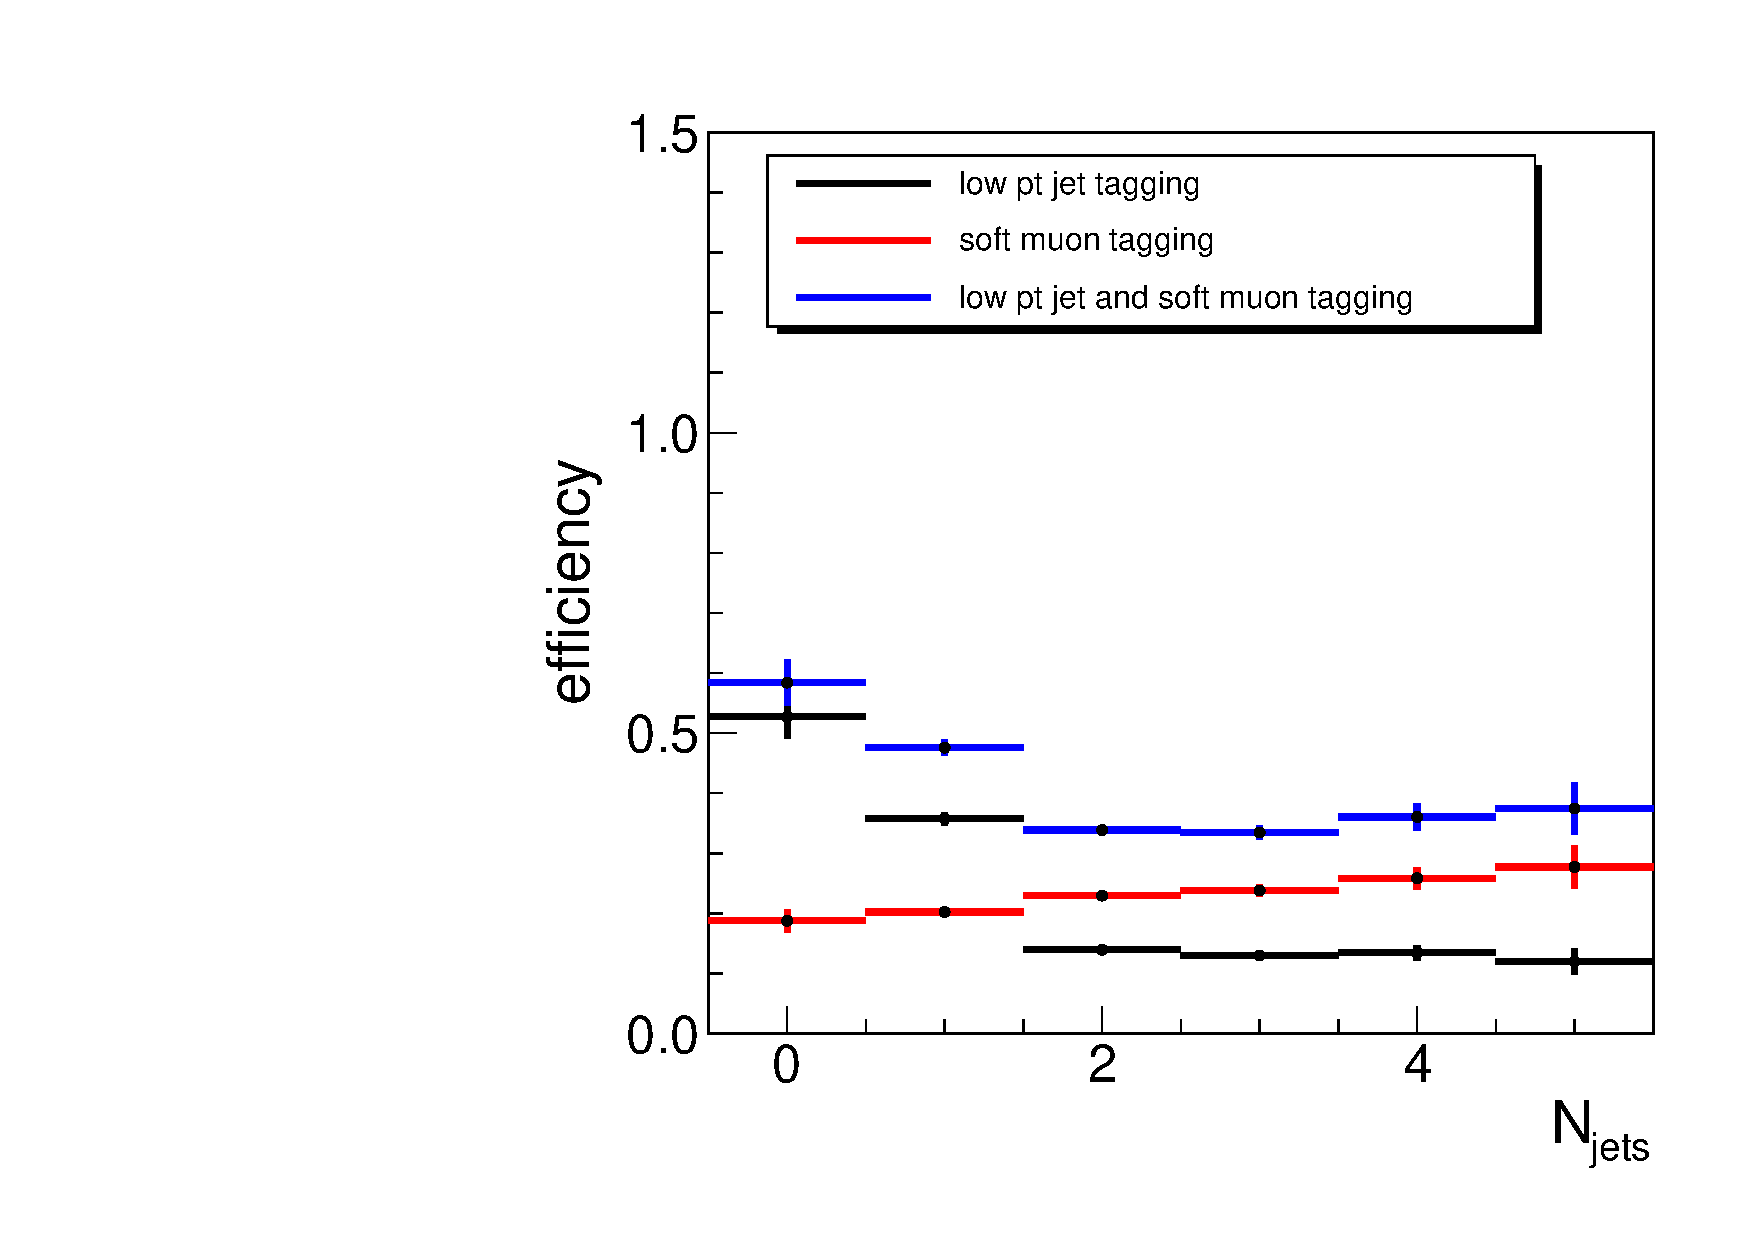
\includegraphics[width=0.60\textwidth]{figures/btag_njets_lowpttagging.pdf}
\caption{Tagging efficiency for low $\pt$ jets, soft muon tagging efficiency 
and the combination of both of them for top simulated events as a function 
of the number of reconstructed jets in top events after applying the 
$\WW$-like selection.}
\label{fig:btag_njets_lowpttagging}
\end{center}
\end{figure}

%
% ONE JET BIN
%
\subsubsection{1-Jet Bin Method}
To measure the tagging efficiency in the 1-jet bin we use top events 
with two reconstructed jets as the control sample. 
The expected tagging efficiency in simulated $t\bar{t}$ events after the $WW$ preselection
is shown using all jets and soft-muons and for the highest $\pt$ jet only
as a function of the number of counted jets in Figure~\ref{fig:btag_njets_highestptjet}.
The tagging efficiency for the highest $\pt$ jet is approximately
the same for the 1-jet and 2-jet bins. Therefore, we propose to use the 
tagging on the highest $\pt$ jet and measure the tagging efficiency in
the 2-jet bin. 

\begin{figure}[!htbp]
\begin{center}
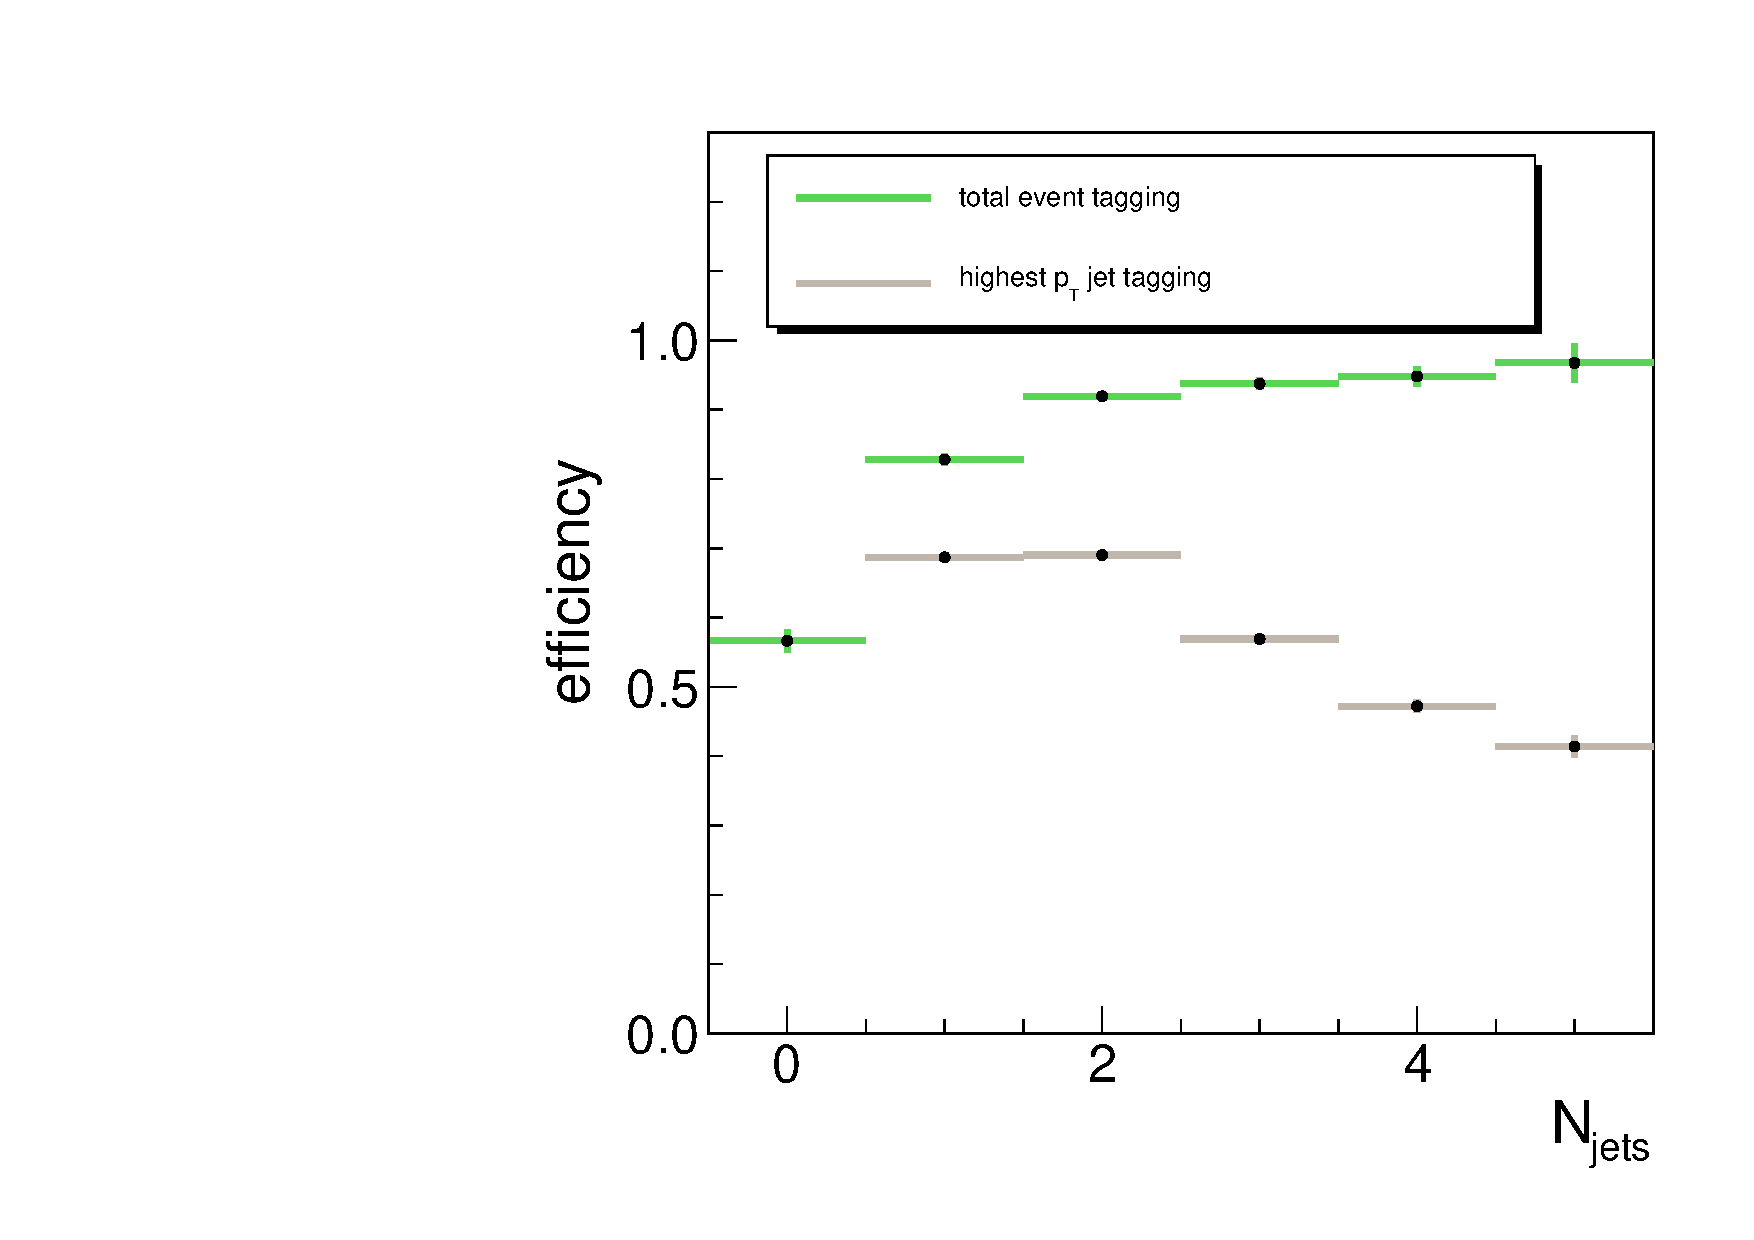
\includegraphics[width=0.55\textwidth]{figures/btag_njets_highestptjet.pdf}
\caption{Total tagging efficiency and tagging efficiency for the highest
$\pt$ jet for simulated top events as a function of the number of reconstructed
jets in top events after applying the $\WW$-like selection.}
\label{fig:btag_njets_highestptjet}
\end{center}
\end{figure}

The residual number of top events in the 1-jet bin is then given by,
$${N_{no~tagged}^{1-jet} = N_{tagged}^{1-jet} \times (1-\epsilon_{highest~\pt~jet})/\epsilon_{highest~\pt~jet}},$$
where $N_{tagged}^{1-jet}$ is the number of events where the counted jet is
tagged and none of the other non-counted jets are tagged, and $\epsilon_{highest~\pt~jet}$ is the 
tagging efficiency for the highest $p_{T}$ jet measured from the 2-jet bin.
The closure test, comparing the estimate using this procedure with 
the simulation, gives agreement to within $1\%$.

%
% VBF
% 
\subsubsection{2-Jet Bin Method}
Estimation of the top background in the 2-jet bin is complicated due to 
the additional requirements applied to the jets to
select $qqH$-like events. The tagging effiency for the selected jets 
after applying such selection is smaller than that in the inclusive 
2-jet bin sample, since the selection enhances events with forward 
jets, which have lower tagging efficiency.

The proposed method is to measure the tagging efficiency of the most central 
jet in the event as a function of its $\pt$ and $\eta$ in an inclusive top 
enriched control sample, and then apply that rate to fully selected events 
where the most central jet is top tagged. In this way the 
possible kinematical differences between the control and signal regions 
are taken into account.

Therefore, the residual number of top events in the 2-jet bin after applying the full 
$qqH$-like is given by,
$${N_{non~tagged}^{qqH} = N_{tagged}^{qqH} \times (1-\epsilon_{central~jet})/\epsilon_{central~jet}},$$
where $N_{no~tagged/tagged}^{qqH}$ is the number non-tagged/tagged events using 
the most central jet, and $\epsilon_{central~jet}$ is the 
tagging efficiency as a function of $\pt$ and $\eta$ of the jet. The comparison of the 
$|\eta|$ distribution of the most central jet in top events after applying the $qqH$-like selection between the simulation and 
the prediction using top-tagged events is shown in Figure~\ref{fig:vbf_btagprediction_jetmin}, where 
good agreement in shape and normalization is observed in the region $|\eta|<2.5$. A small correction 
of about 10\% in the yield must be included in the prediction to take into account the fraction 
of top events where the most central jet is outside the tracker acceptance.

\begin{figure}[!htbp]
\begin{center}
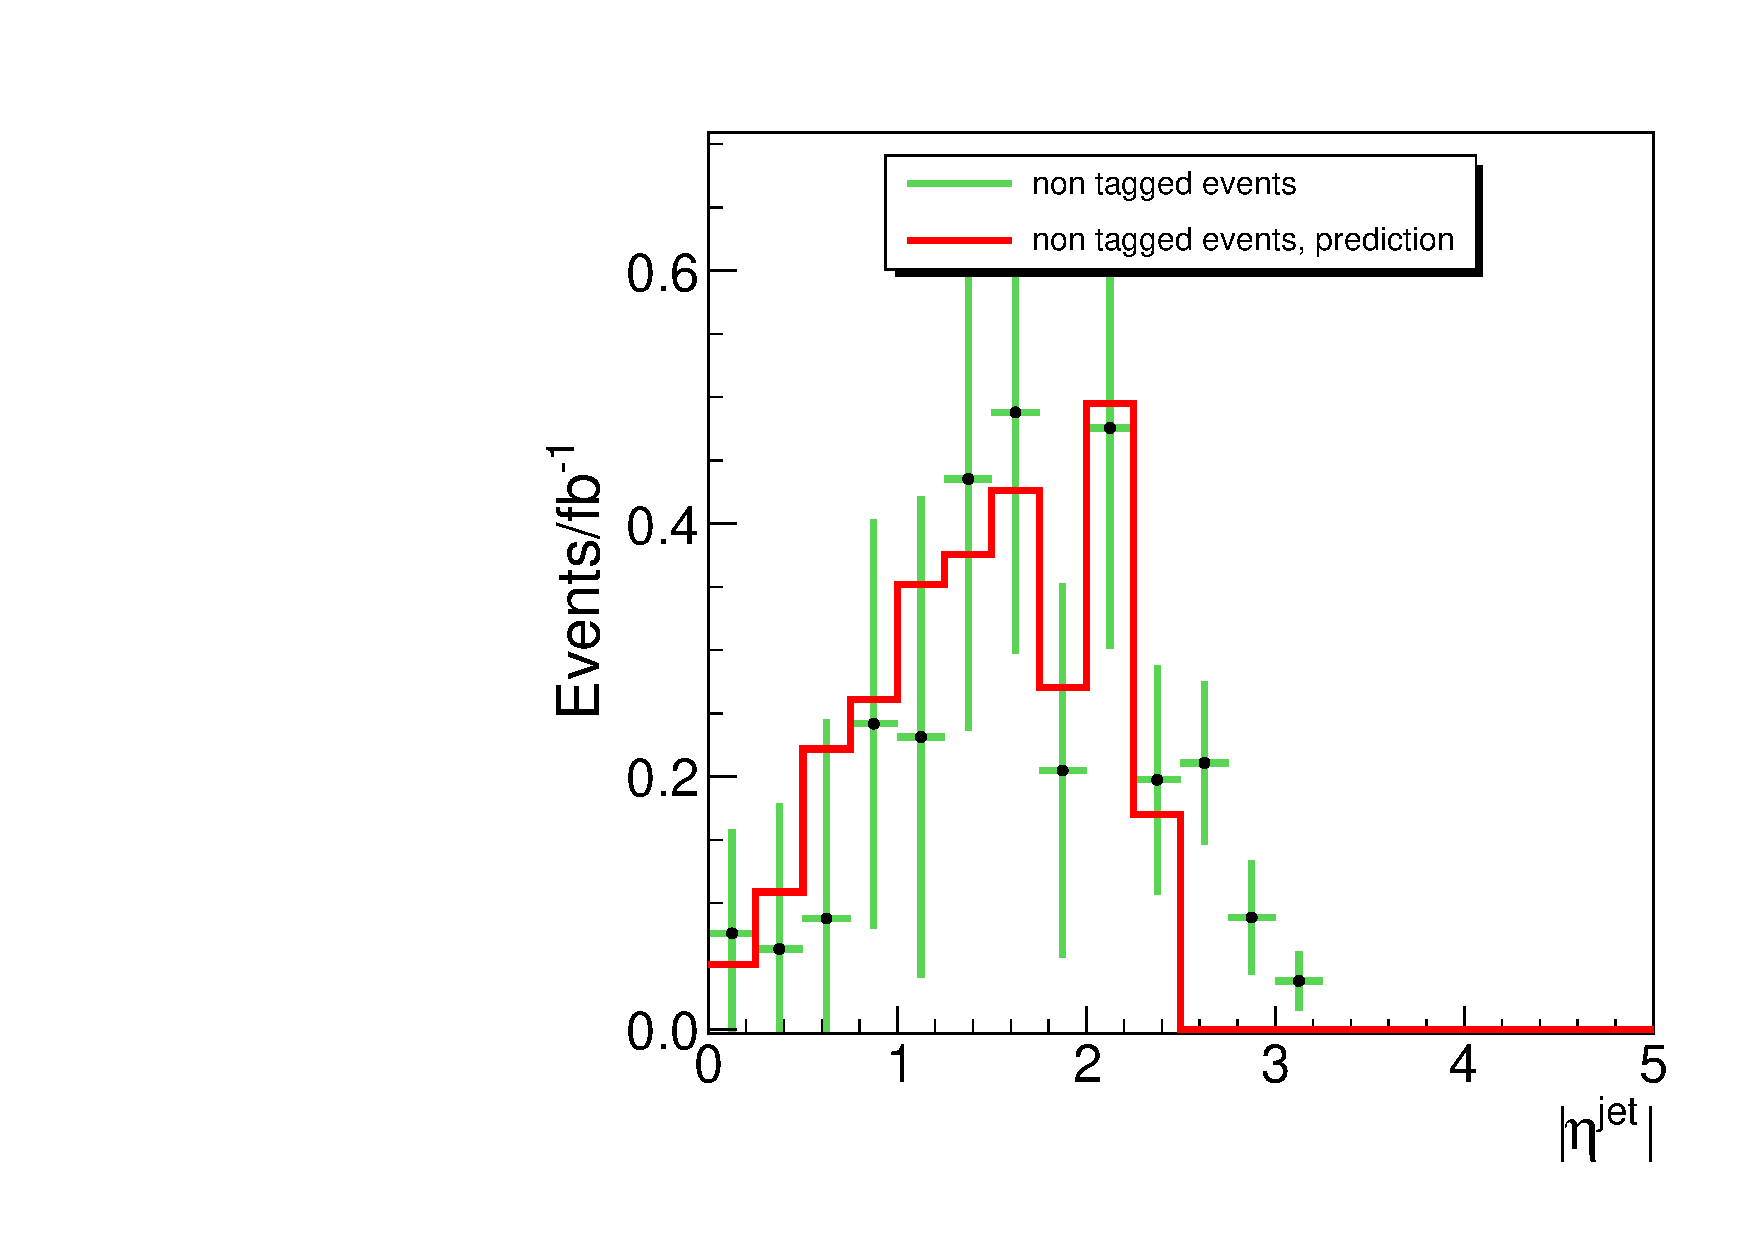
\includegraphics[width=0.65\textwidth]{figures/vbf_btagprediction_jetmin.pdf}
\caption{$|\eta|$ distribution of the most central jet in top events after 
applying the $qqH$-like selection. Comparison between the simulation and 
the prediction using top-tagged events.}
\label{fig:vbf_btagprediction_jetmin}
\end{center}
\end{figure}

%jets and soft muons in the event, which has little correlation 
%with the two tagging jets. The tagging efficiency for the combination of 
%low $\pt$ jets and soft muons after and before applying the $qqH$-like 
%selection, and after and before requiring that the two highest $\pt$ jets 
%in the event are not tagged is shown in 
%Figure~\ref{fig:btag_njets_vbfcuts}. We see that just by requiring the two 
%highest $\pt$ jets in the event not tagged, the agreement in the 2-jet 
%bin is rather good.

%The proposed method is to measure the tagging efficiency using low $\pt$ 
%jets and soft muons in the event, which has little correlation 
%with the two tagging jets. The tagging efficiency for the combination of 
%low $\pt$ jets and soft muons after and before applying the $qqH$-like 
%selection, and after and before requiring that the two highest $\pt$ jets 
%in the event are not tagged is shown in 
%Figure~\ref{fig:btag_njets_vbfcuts}. We see that just by requiring the two 
%highest $\pt$ jets in the event not tagged, the agreement in the 2-jet 
%bin is rather good.

%\begin{figure}[!htbp]
%\begin{center}
%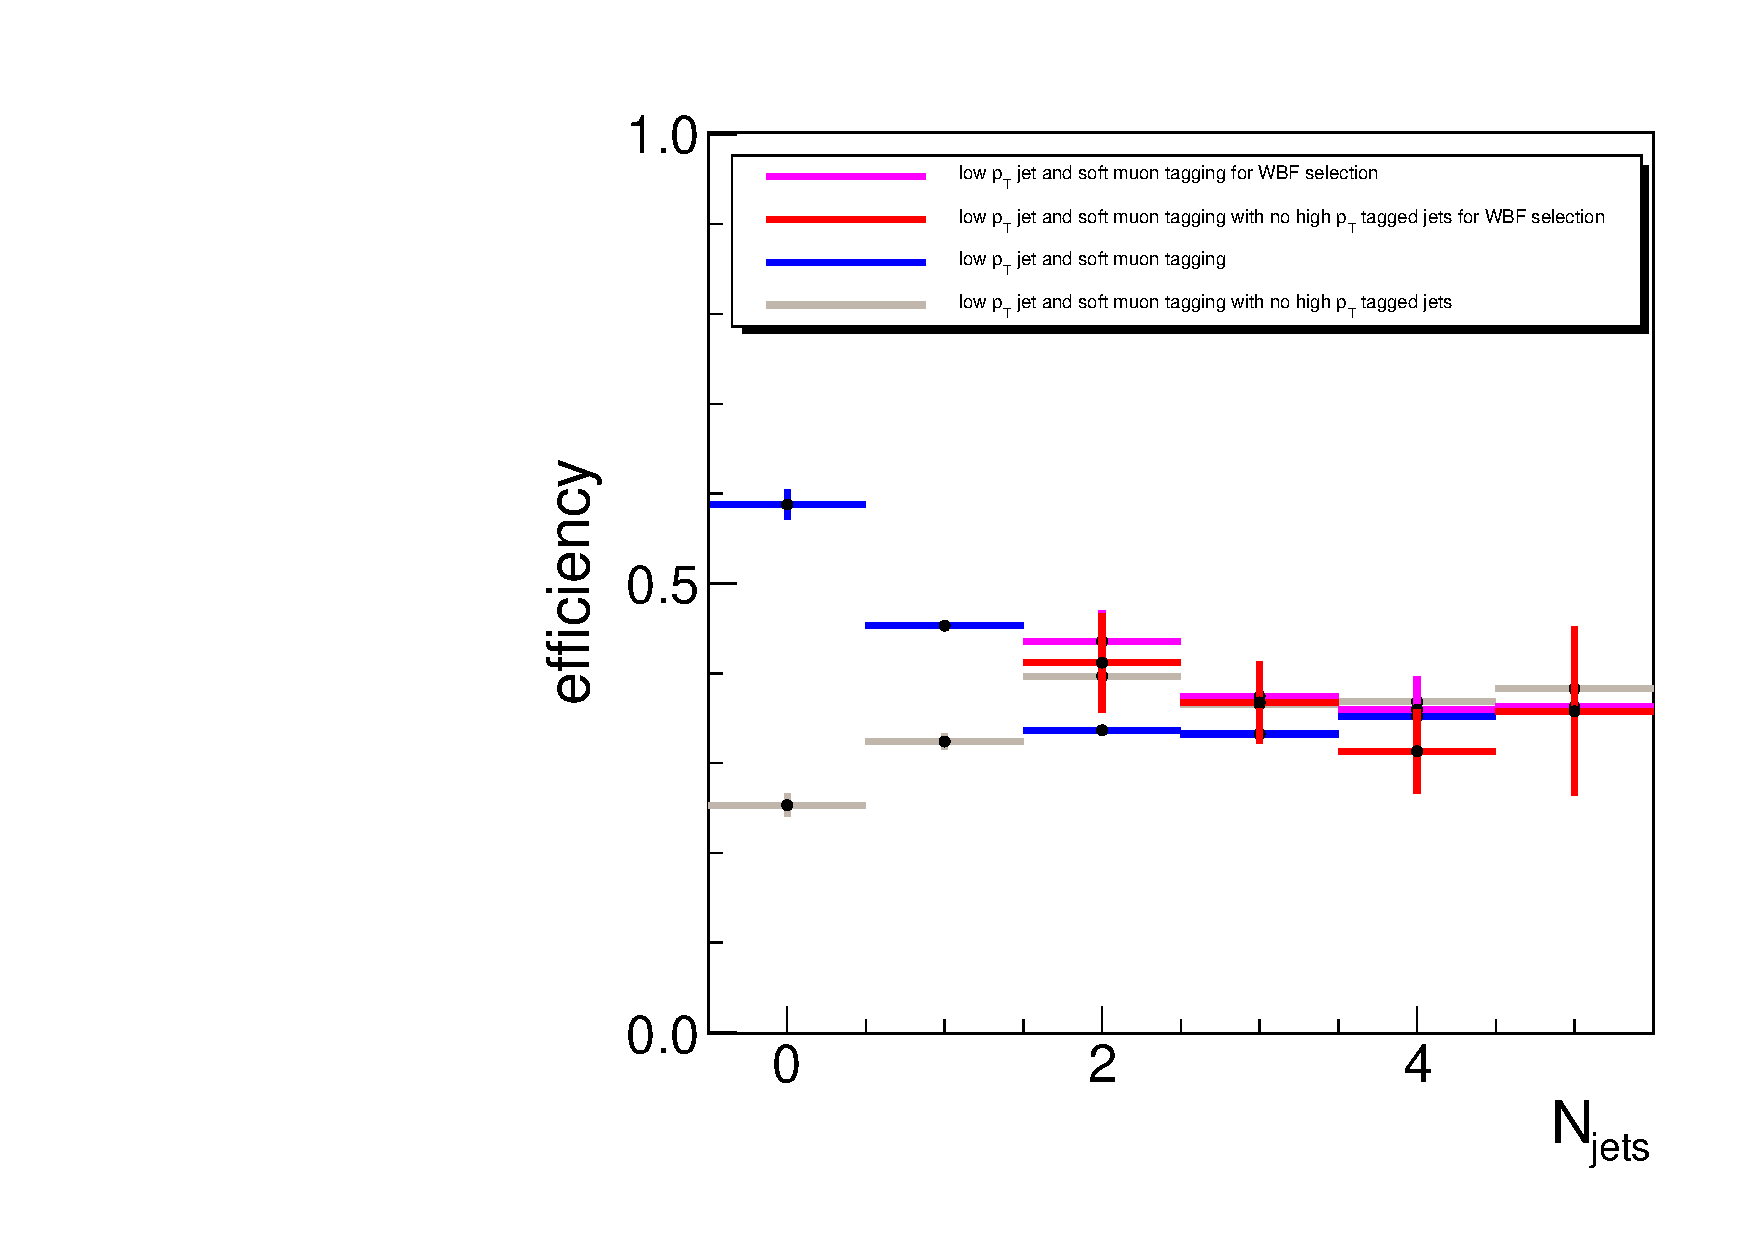
\includegraphics[width=0.65\textwidth]{figures/btag_njets_vbfcuts.pdf}
%\caption{Tagging efficiency for the combination of 
%low $\pt$ jets and soft muons after and before applying the $qqH$-like 
%selection, and after and before requiring that the two highest $\pt$ jets 
%in the event are not tagged.}
%\label{fig:btag_njets_vbfcuts}
%\end{center}
%\end{figure}

%Therefore, the residual number of top events in the 2-jet bin after applying the full 
%$qqH$-like is given by,
%$${N_{no~tagged}^{qqH} = N_{tagged}^{qqH} \times (1-\epsilon_{soft~jets})/\epsilon_{soft~jets}},$$
%where $N_{no~tagged/tagged}^{qqH}$ is the number of events where the event is no-tagged/tagged by either low $\pt$ 
%jets or soft muons, and $\epsilon_{soft~jets}$ is the 
%tagging efficiency for low $\pt$ jets and soft muons measured from the 2-jet bin for events where the two 
%highest $\pt$ jets in the event not $b$-tagged. The closure test, comparing the estimate using 
%this procedure with the simulation, gives agreement to within $5\%$.

%
% ON DATA
%
\subsubsection{Data Results}
This section describes the tagging efficiency results obtained in data, 
and the comparison of the residual background predictions obtained from
the methods described above with simulation expectations.

The tagging efficiency for the combination of low $\pt$ jets 
and soft muons as a function of the number of counted jets on data and 
simulation is shown in Figure~\ref{fig:btag_njets_lowpttagging_data}. 
The total tagging efficiency as a function of the number of reconstructed jets on data 
and simulation is shown in Figure~\ref{fig:btag_njets_totaltagging_data}. 
The tagging efficiency for the leading jet $\pt$ as a function of the number of 
reconstructed jets on data and simulation is shown in 
Figure~\ref{fig:btag_njets_highestptjet_data}. 
In all cases a reasonable agreement is found between the data 
and the simulation, although the statistical uncertainty is large.

\begin{figure}[!htbp]
\begin{center}
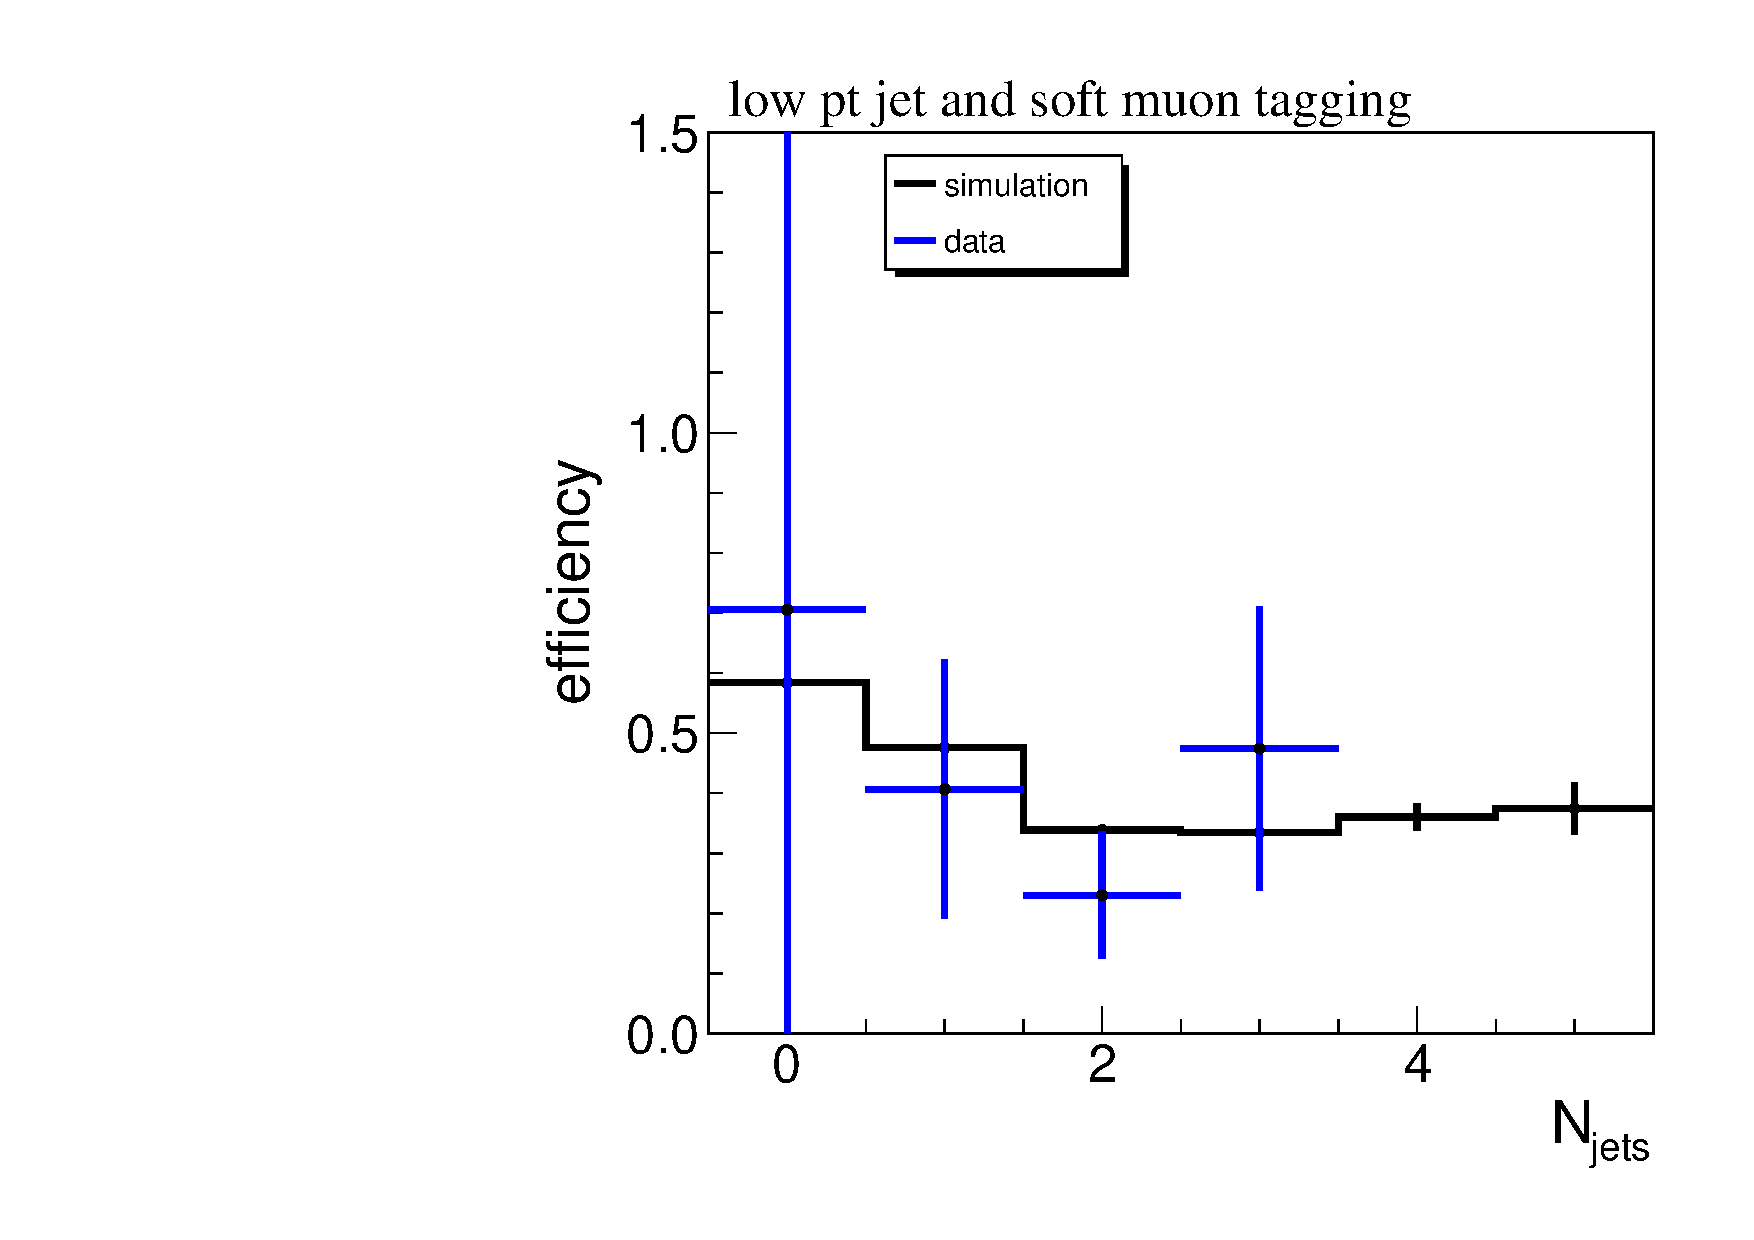
\includegraphics[width=0.55\textwidth]{figures/btag_njets_lowpttagging_data.pdf}
\caption{Tagging efficiency for the combination of low $\pt$ jets and soft muons 
as a function of the number of counted jets after applying 
the $\WW$-like selection on data and simulation.}
\label{fig:btag_njets_lowpttagging_data}
\end{center}
\end{figure}

\begin{figure}[!htbp]
\begin{center}
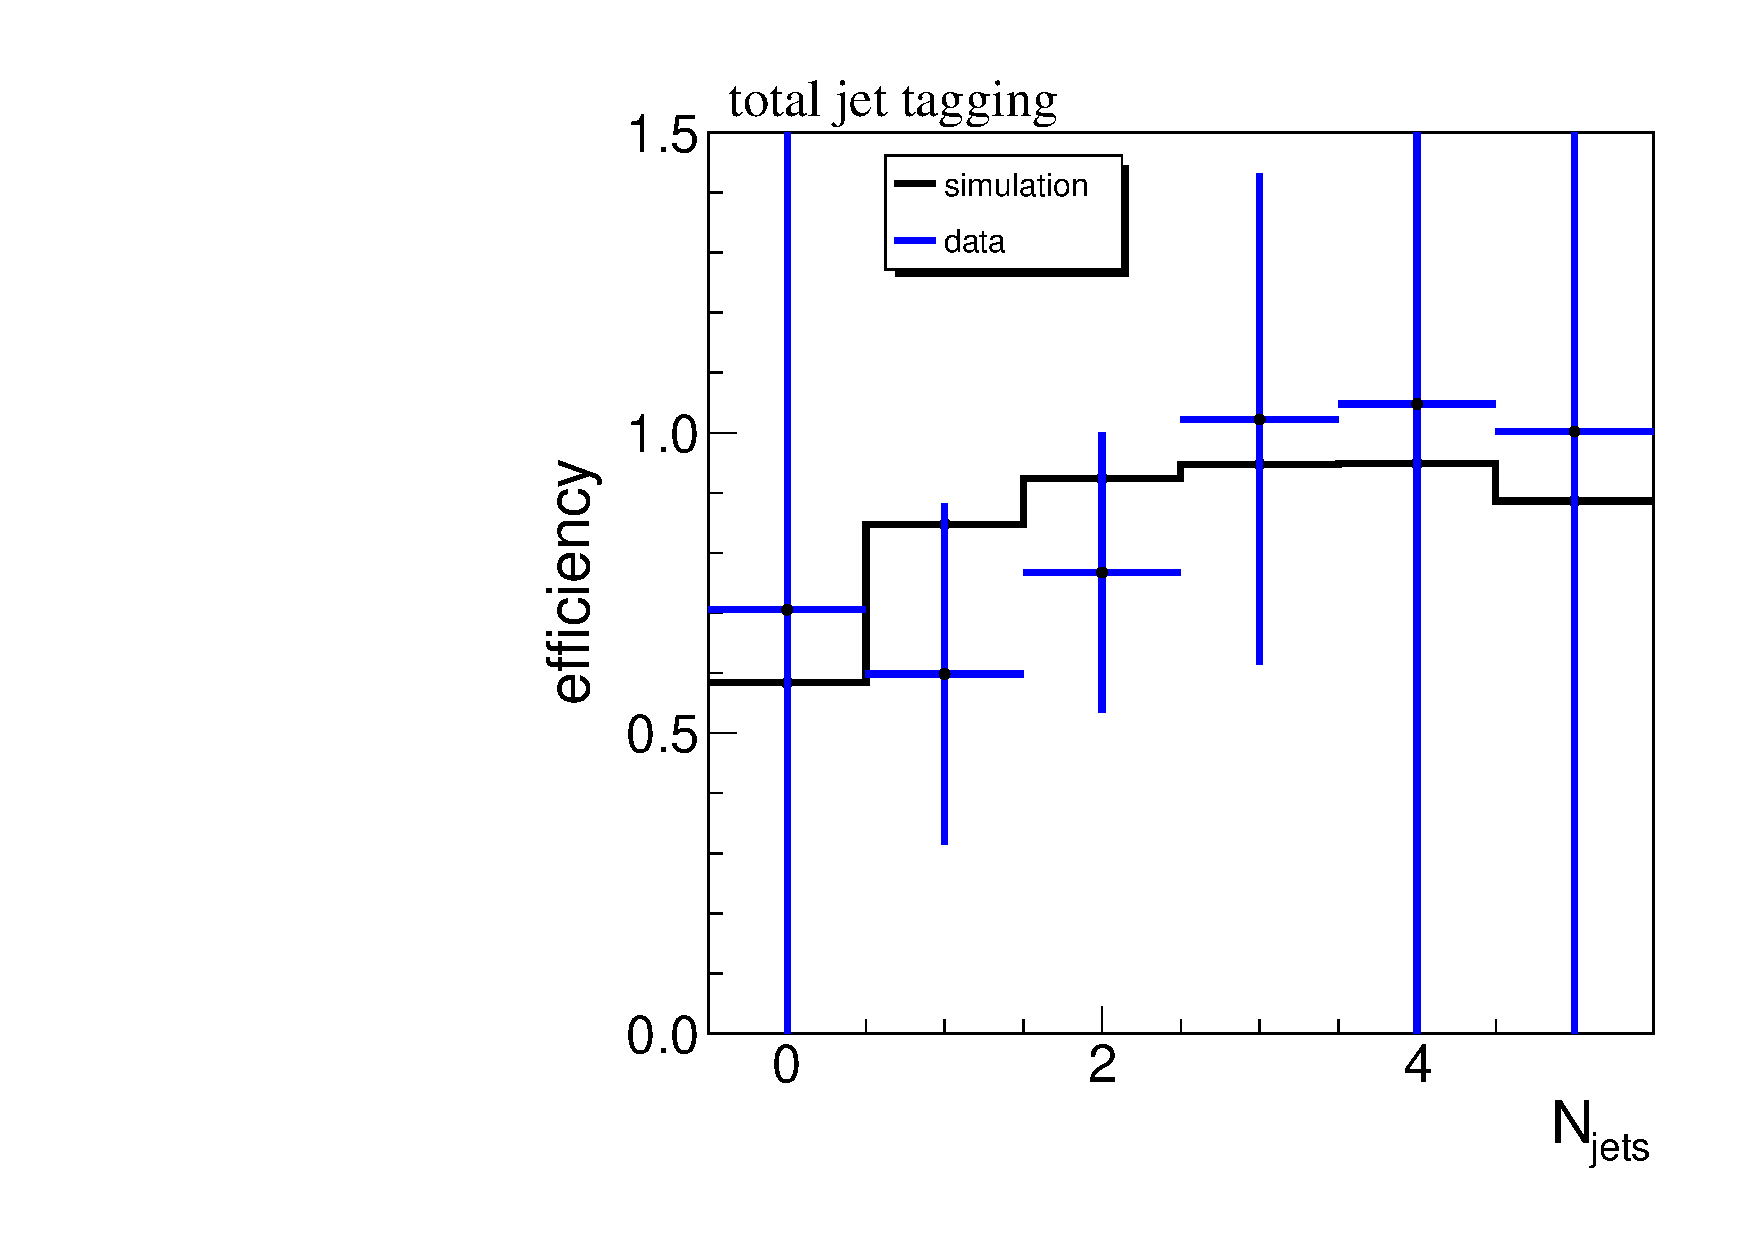
\includegraphics[width=0.55\textwidth]{figures/btag_njets_totaltagging_data.pdf}
\caption{The total tagging efficiency as a function of the number of counted 
jets after applying the $\WW$-like selection on data and simulation.}
\label{fig:btag_njets_totaltagging_data}
\end{center}
\end{figure}

\begin{figure}[!htbp]
\begin{center}
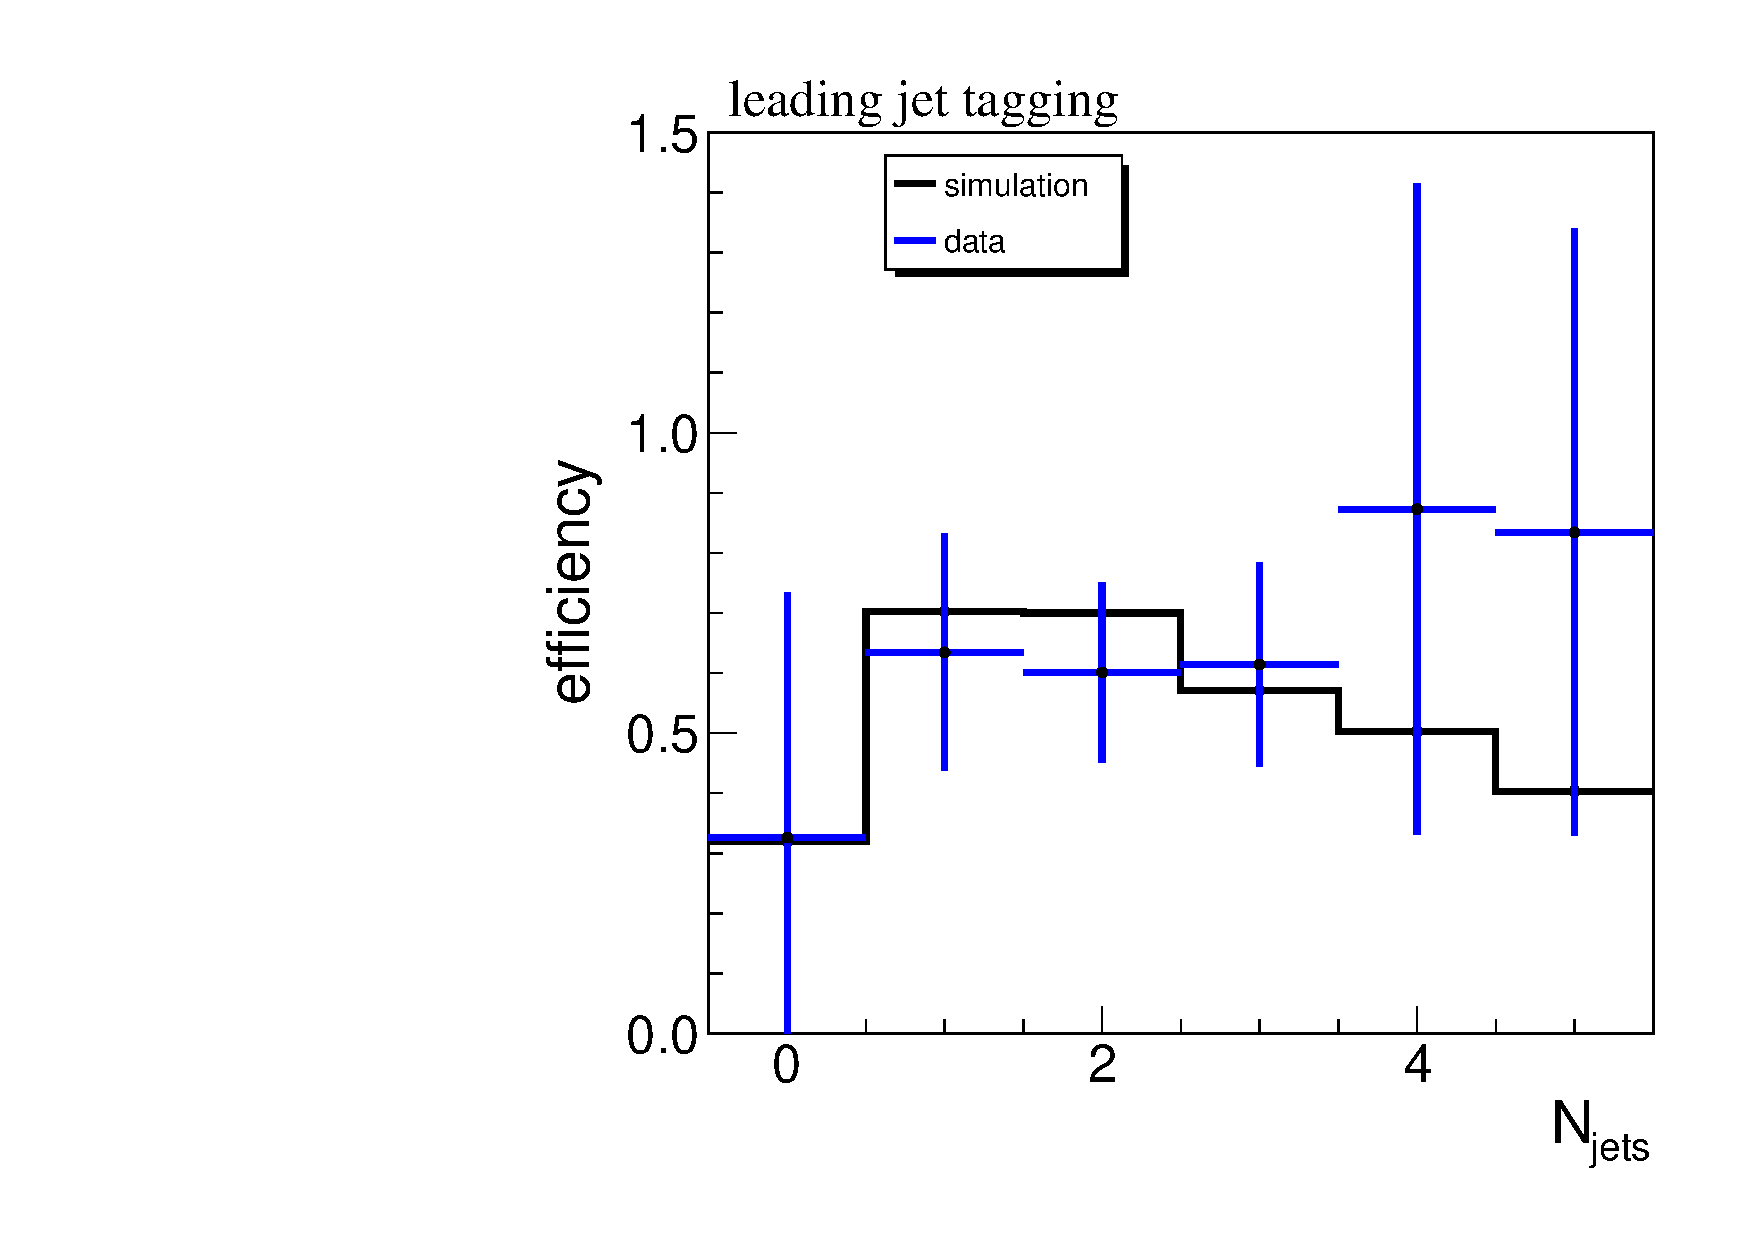
\includegraphics[width=0.55\textwidth]{figures/btag_njets_highestptjet_data.pdf}
\caption{Tagging efficiency for the leading jet $\pt$ as a function of the number of counted 
jets after applying the $\WW$-like selection on data and simulation.}
\label{fig:btag_njets_highestptjet_data}
\end{center}
\end{figure}
